\documentclass{standalone}
\usepackage{tikz}
\usetikzlibrary{patterns, positioning}


\begin{document}
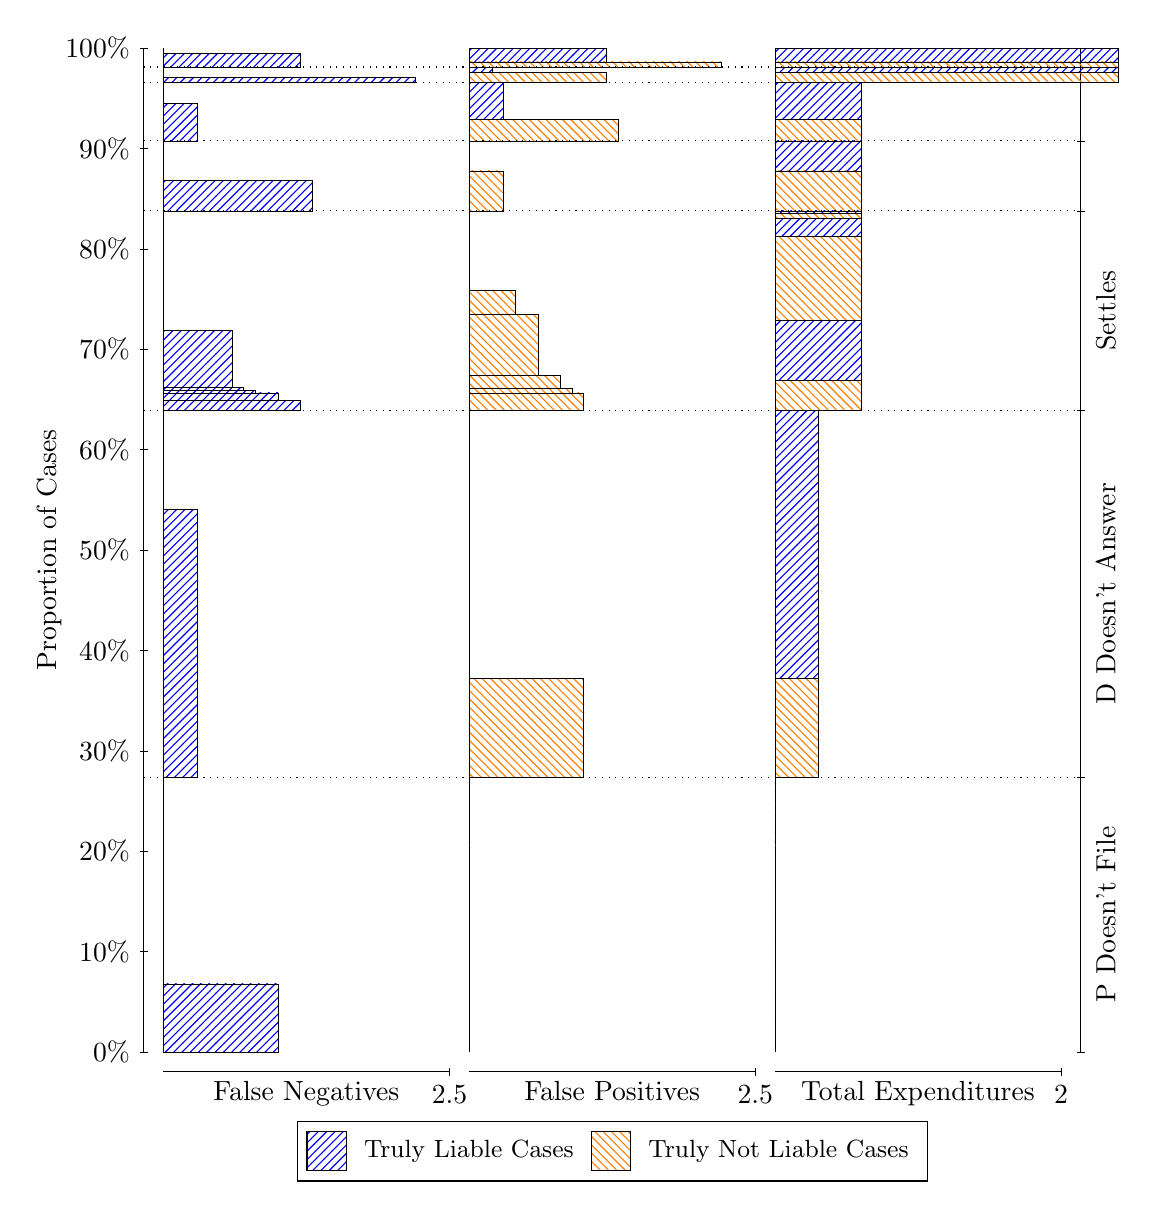
\begin{tikzpicture}
\draw[black, very thin] (1.5,1.75) -- (1.5,14.5);
\node[rotate=90, text=black, anchor=center] at (0.3, 8.125) {Proportion of Cases};
\draw[black, very thin] (1.45,1.75) -- (1.55,1.75);
\node[text=black, anchor=east] at (1.45, 1.75) {0\%};
\draw[black, very thin] (1.45,3.025) -- (1.55,3.025);
\node[text=black, anchor=east] at (1.45, 3.025) {10\%};
\draw[black, very thin] (1.45,4.3) -- (1.55,4.3);
\node[text=black, anchor=east] at (1.45, 4.3) {20\%};
\draw[black, very thin] (1.45,5.575) -- (1.55,5.575);
\node[text=black, anchor=east] at (1.45, 5.575) {30\%};
\draw[black, very thin] (1.45,6.85) -- (1.55,6.85);
\node[text=black, anchor=east] at (1.45, 6.85) {40\%};
\draw[black, very thin] (1.45,8.125) -- (1.55,8.125);
\node[text=black, anchor=east] at (1.45, 8.125) {50\%};
\draw[black, very thin] (1.45,9.4) -- (1.55,9.4);
\node[text=black, anchor=east] at (1.45, 9.4) {60\%};
\draw[black, very thin] (1.45,10.675) -- (1.55,10.675);
\node[text=black, anchor=east] at (1.45, 10.675) {70\%};
\draw[black, very thin] (1.45,11.95) -- (1.55,11.95);
\node[text=black, anchor=east] at (1.45, 11.95) {80\%};
\draw[black, very thin] (1.45,13.225) -- (1.55,13.225);
\node[text=black, anchor=east] at (1.45, 13.225) {90\%};
\draw[black, very thin] (1.45,14.5) -- (1.55,14.5);
\node[text=black, anchor=east] at (1.45, 14.5) {100\%};

\draw[black, very thin] (13.4,1.75) -- (13.4,14.5);
\draw[black, very thin] (13.35,1.75) -- (13.45,1.75);
\node[anchor=west] at (13.35, 1.75) {};
\draw[black, very thin] (13.35,5.2405) -- (13.45,5.2405);
\node[anchor=west] at (13.35, 5.2405) {};
\draw[black, very thin] (13.35,9.8972) -- (13.45,9.8972);
\node[anchor=west] at (13.35, 9.8972) {};
\draw[black, very thin] (13.35,12.433) -- (13.45,12.433);
\node[anchor=west] at (13.35, 12.433) {};
\draw[black, very thin] (13.35,13.322) -- (13.45,13.322);
\node[anchor=west] at (13.35, 13.322) {};
\draw[black, very thin] (13.35,14.061) -- (13.45,14.061);
\node[anchor=west] at (13.35, 14.061) {};
\draw[black, very thin] (13.35,14.259) -- (13.45,14.259);
\node[anchor=west] at (13.35, 14.259) {};
\draw[black, very thin] (13.35,14.5) -- (13.45,14.5);
\node[anchor=west] at (13.35, 14.5) {};

\draw[black, very thin, pattern color=blue, pattern=north east lines] (1.75,1.75) rectangle (3.2033,2.6151);
\draw[black, very thin, pattern color=orange, pattern=north west lines] (1.75,2.6151) rectangle (1.75,5.2405);
\draw[black, very thin, pattern color=blue, pattern=north east lines] (1.75,5.2405) rectangle (2.186,8.6437);
\draw[black, very thin, pattern color=orange, pattern=north west lines] (1.75,8.6437) rectangle (1.75,9.8972);
\draw[black, very thin, pattern color=blue, pattern=north east lines] (1.75,9.8972) rectangle (3.494,10.022);
\draw[black, very thin, pattern color=blue, pattern=north east lines] (1.75,10.022) rectangle (3.2033,10.121);
\draw[black, very thin, pattern color=blue, pattern=north east lines] (1.75,10.121) rectangle (2.9127,10.151);
\draw[black, very thin, pattern color=blue, pattern=north east lines] (1.75,10.151) rectangle (2.7673,10.186);
\draw[black, very thin, pattern color=blue, pattern=north east lines] (1.75,10.186) rectangle (2.622,10.912);
\draw[black, very thin, pattern color=orange, pattern=north west lines] (1.75,10.912) rectangle (1.75,12.433);
\draw[black, very thin, pattern color=blue, pattern=north east lines] (1.75,12.433) rectangle (3.6393,12.815);
\draw[black, very thin, pattern color=orange, pattern=north west lines] (1.75,12.815) rectangle (1.75,13.322);
\draw[black, very thin, pattern color=blue, pattern=north east lines] (1.75,13.322) rectangle (2.186,13.792);
\draw[black, very thin, pattern color=orange, pattern=north west lines] (1.75,13.792) rectangle (1.75,14.061);
\draw[black, very thin, pattern color=blue, pattern=north east lines] (1.75,14.061) rectangle (4.9473,14.127);
\draw[black, very thin, pattern color=orange, pattern=north west lines] (1.75,14.127) rectangle (1.75,14.259);
\draw[black, very thin, pattern color=blue, pattern=north east lines] (1.75,14.259) rectangle (3.494,14.434);
\draw[black, very thin, pattern color=orange, pattern=north west lines] (1.75,14.434) rectangle (1.75,14.5);
\draw[black, very thin, pattern color=orange, pattern=north west lines] (5.6333,1.75) rectangle (5.6333,4.3754);
\draw[black, very thin, pattern color=blue, pattern=north east lines] (5.6333,4.3754) rectangle (5.6333,5.2405);
\draw[black, very thin, pattern color=orange, pattern=north west lines] (5.6333,5.2405) rectangle (7.0867,6.494);
\draw[black, very thin, pattern color=blue, pattern=north east lines] (5.6333,6.494) rectangle (5.6333,9.8972);
\draw[black, very thin, pattern color=orange, pattern=north west lines] (5.6333,9.8972) rectangle (7.0867,10.12);
\draw[black, very thin, pattern color=orange, pattern=north west lines] (5.6333,10.12) rectangle (6.9413,10.182);
\draw[black, very thin, pattern color=orange, pattern=north west lines] (5.6333,10.182) rectangle (6.796,10.343);
\draw[black, very thin, pattern color=orange, pattern=north west lines] (5.6333,10.343) rectangle (6.5053,11.118);
\draw[black, very thin, pattern color=orange, pattern=north west lines] (5.6333,11.118) rectangle (6.2147,11.418);
\draw[black, very thin, pattern color=blue, pattern=north east lines] (5.6333,11.418) rectangle (5.6333,12.433);
\draw[black, very thin, pattern color=orange, pattern=north west lines] (5.6333,12.433) rectangle (6.0693,12.94);
\draw[black, very thin, pattern color=blue, pattern=north east lines] (5.6333,12.94) rectangle (5.6333,13.322);
\draw[black, very thin, pattern color=orange, pattern=north west lines] (5.6333,13.322) rectangle (7.5227,13.592);
\draw[black, very thin, pattern color=blue, pattern=north east lines] (5.6333,13.592) rectangle (6.0693,14.061);
\draw[black, very thin, pattern color=orange, pattern=north west lines] (5.6333,14.061) rectangle (7.3773,14.193);
\draw[black, very thin, pattern color=blue, pattern=north east lines] (5.6333,14.193) rectangle (5.924,14.259);
\draw[black, very thin, pattern color=orange, pattern=north west lines] (5.6333,14.259) rectangle (8.8307,14.325);
\draw[black, very thin, pattern color=blue, pattern=north east lines] (5.6333,14.325) rectangle (7.3773,14.5);
\draw[black, very thin, pattern color=orange, pattern=north west lines] (9.5167,1.75) rectangle (9.5167,4.3754);
\draw[black, very thin, pattern color=blue, pattern=north east lines] (9.5167,4.3754) rectangle (9.5167,5.2405);
\draw[black, very thin, pattern color=orange, pattern=north west lines] (9.5167,5.2405) rectangle (10.062,6.494);
\draw[black, very thin, pattern color=blue, pattern=north east lines] (9.5167,6.494) rectangle (10.062,9.8972);
\draw[black, very thin, pattern color=orange, pattern=north west lines] (9.5167,9.8972) rectangle (10.607,10.281);
\draw[black, very thin, pattern color=blue, pattern=north east lines] (9.5167,10.281) rectangle (10.607,11.037);
\draw[black, very thin, pattern color=orange, pattern=north west lines] (9.5167,11.037) rectangle (10.607,12.112);
\draw[black, very thin, pattern color=blue, pattern=north east lines] (9.5167,12.112) rectangle (10.607,12.336);
\draw[black, very thin, pattern color=orange, pattern=north west lines] (9.5167,12.336) rectangle (10.607,12.398);
\draw[black, very thin, pattern color=blue, pattern=north east lines] (9.5167,12.398) rectangle (10.607,12.433);
\draw[black, very thin, pattern color=orange, pattern=north west lines] (9.5167,12.433) rectangle (10.607,12.94);
\draw[black, very thin, pattern color=blue, pattern=north east lines] (9.5167,12.94) rectangle (10.607,13.322);
\draw[black, very thin, pattern color=orange, pattern=north west lines] (9.5167,13.322) rectangle (10.607,13.592);
\draw[black, very thin, pattern color=blue, pattern=north east lines] (9.5167,13.592) rectangle (10.607,14.061);
\draw[black, very thin, pattern color=orange, pattern=north west lines] (9.5167,14.061) rectangle (13.877,14.193);
\draw[black, very thin, pattern color=blue, pattern=north east lines] (9.5167,14.193) rectangle (13.877,14.259);
\draw[black, very thin, pattern color=orange, pattern=north west lines] (9.5167,14.259) rectangle (13.877,14.325);
\draw[black, very thin, pattern color=blue, pattern=north east lines] (9.5167,14.325) rectangle (13.877,14.5);
\draw[black, dotted] (1.5,5.2405) -- (13.4,5.2405);
\draw[black, dotted] (1.5,9.8972) -- (13.4,9.8972);
\draw[black, dotted] (1.5,12.433) -- (13.4,12.433);
\draw[black, dotted] (1.5,13.322) -- (13.4,13.322);
\draw[black, dotted] (1.5,14.061) -- (13.4,14.061);
\draw[black, dotted] (1.5,14.259) -- (13.4,14.259);
\draw[black, very thin] (1.75,1.5) -- (5.3833,1.5);
\node[text=black, anchor=north] at (3.5667, 1.5) {False Negatives};
\draw[black, very thin] (5.3833,1.45) -- (5.3833,1.55);
\node[text=black, anchor=north] at (5.3833, 1.45) {2.5};

\draw[black, very thin] (5.6333,1.5) -- (9.2667,1.5);
\node[text=black, anchor=north] at (7.45, 1.5) {False Positives};
\draw[black, very thin] (9.2667,1.45) -- (9.2667,1.55);
\node[text=black, anchor=north] at (9.2667, 1.45) {2.5};

\draw[black, very thin] (9.5167,1.5) -- (13.15,1.5);
\node[text=black, anchor=north] at (11.333, 1.5) {Total Expenditures};
\draw[black, very thin] (13.15,1.45) -- (13.15,1.55);
\node[text=black, anchor=north] at (13.15, 1.45) {2};

\node[text=black, centered, rotate=90] at (13.72, 3.4953) {P Doesn't File};
\node[text=black, centered, rotate=90] at (13.72, 7.5688) {D Doesn't Answer};
\node[text=black, centered, rotate=90] at (13.72, 11.165) {Settles};





\draw (7.449999999999999,1.5) node[draw=none] (baseCoordinate) {};
\begin{scope}[align=center]
        \matrix[scale=0.5, draw=black, below=0.5cm of baseCoordinate, nodes={draw}, column sep=0.1cm]{
            \node[rectangle, draw, minimum width=0.5cm, minimum height=0.5cm, pattern color=blue, pattern=north east lines] {}; &
            \node[draw=none, font=\small, text=black] (B) {Truly Liable Cases}; &
            \node[rectangle, draw, minimum width=0.5cm, minimum height=0.5cm, pattern color=orange, pattern=north west lines] {}; &
            \node[draw=none, font=\small, text=black] (B) {Truly Not Liable Cases}; \\
            };
\end{scope}

\end{tikzpicture}
\end{document}